\documentclass{article}
\usepackage{amsmath}
\usepackage{amssymb}
\usepackage{hyperref}
\usepackage{graphicx}
\usepackage{xcolor}
\usepackage[
  left=1cm,
  right=1cm,
  top=2cm,
  bottom=2cm,
]{geometry}

\begin{document}

\begin{center}
    Bei Krankheit oder Verhinderung, Aufgaben per Mail:\\
    \textbf{peter.gierss@ihfg.uni-stuttgart.de}
\end{center}

\section*{Woche 1}
\subsection*{Aufgabe 1}
\begin{itemize}
    \item Reibungselektrizität: PVC Rohr mit Stoff \textcolor{gray}{(Elektronen werden abgestreift)}
    \item Elektrische Kraft: Kondensation
    \item Influenz: Induzierter Dipol
    \item Chemische Vorgänge: Elektrolyse
    \item Strahlung: Zerfall
    \item Ionisation
    \item Mechanisch trennen
\end{itemize}
\begin{equation*}
    \vec{F_C} = \frac{1}{4\pi\varepsilon_0}\cdot\frac{q_1q_2}{r^2}\hat{r} =\frac{1}{4\pi\varepsilon_0}\cdot\frac{q_1q_2}{r^3}r
\end{equation*}

\subsection*{Aufgabe 2}
\begin{center}
    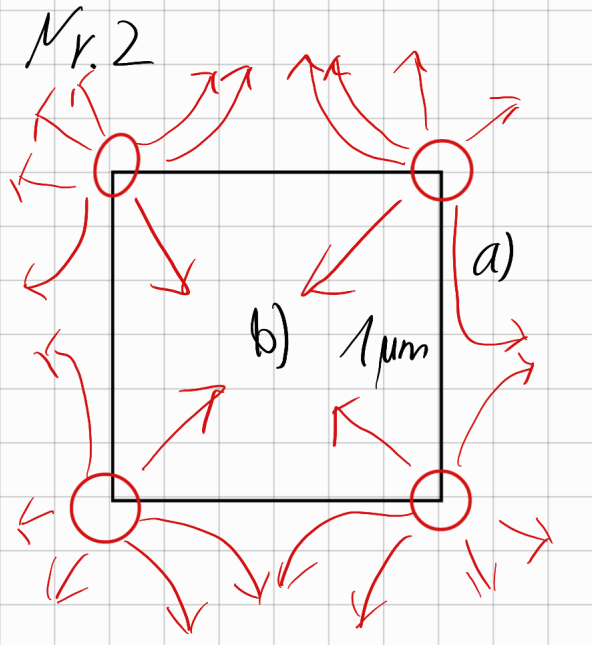
\includegraphics{Abbildungen/Abb.1.png}
\end{center}
\begin{itemize}
    \item[c)] Abstand der Protonen würde gleich bleiben, das ganze System bewegt sich mit.
\end{itemize}
\begin{equation*}
    \vec{F} = \frac{1}{4\pi \varepsilon_0}\cdot\frac{q_1q_2}{r^2} = 1151,94 \mathrm{\frac{V}{m}} 
\end{equation*}
Da:
\begin{equation*}
    \varepsilon_0 = 8,85 \cdot 10^{-12} \mathrm{\frac{As}{Vm}}
\end{equation*}
\begin{equation*}
    \cos(26,57) = \frac{A}{1151,94 \mathrm{\frac{V}{m}}} = 2060,57 \rightarrow \text{Durch 2} \rightarrow 1030,28 \mathrm{\frac{V}{m}}
\end{equation*}
\begin{equation*}
    \vec{F}=\frac{Q^2}{4\pi \varepsilon_0} \left[\frac{1}{a^3}\left(\begin{array}{c}0\\-a\end{array}\right)+\frac{1}{(a\sqrt{2})^3}\left(\begin{array}{c}-a\\-a\end{array}\right)+\frac{1}{a^3}\left(\begin{array}{c}-a\\0\end{array}\right)\right] = 4.42 \cdot 10^{-16} \text{ N } \cdot \frac{1}{\sqrt{2}}\left(\begin{array}{c}-1\\-1\end{array}\right)
\end{equation*}
\begin{equation*}
    \text{3 Proton} \rightarrow 2\vec{F}+\frac{1}{2}\vec{F}=5,75 \cdot 10^{-28} \text{ N}
\end{equation*}

\subsection*{Aufgabe 3}
\begin{center}
    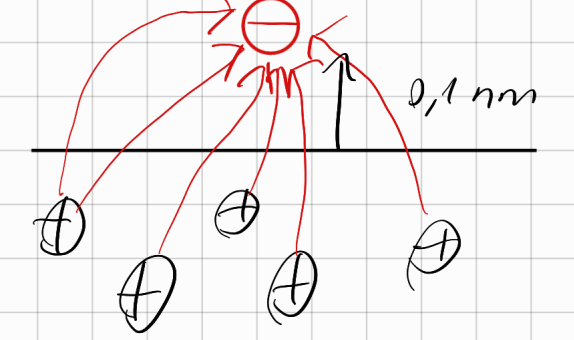
\includegraphics{Abbildungen/Abb.2.png}
\end{center}
\begin{equation*}
    w = \int \vec{F}\,d\vec{s}, \,F=\frac{Q_1Q_2}{4\pi\varepsilon_0}\frac{1}{(2x)^2}
\end{equation*}
\begin{equation*}
    w = \frac{Q_1Q_2}{4\pi\varepsilon_0} \int_{r}^{\infty} \frac{1}{(2x)^2}\,dx = \frac{Q_1Q_2}{4\pi\varepsilon_0} \left[\frac{1}{(2x)^2}\right]^\infty_r = \frac{Q_1Q_2}{4\pi\varepsilon_0} \cdot \frac{1}{4r} = 5.76 \cdot 10^{-19} \text{ J}
\end{equation*}

\subsection*{Aufgabe 4 (T)}
2-Achsiges Koordinatensystem, an den Achsen spiegeln, bis eine Punktsymmetrie zum Ursprung vom Ausgangspunkt entseht, bei einem spitzeren Winkel müssen mehr "Generationen" \textcolor{gray}{(Spiegelladungen)} auftreten, bis die Punktsymmetrie entsteht.

\newpage

\subsection*{Aufgabe 5 (T)}
a) \begin{equation*}
    q_e = -1.6 \cdot 10^{-19} \text{ C}, \, r = 5.29\cdot 10^{-11}\text{ m} q_p = 1.6 \cdot 10^{-19} \text{ C}
\end{equation*}
\begin{equation*}
    F_{el} = \frac{1}{4\pi\varepsilon_0}\frac{|q_e|1_e}{r^2} = -8.2 \cdot 10^{-8} \text{ N}
\end{equation*}
b)
\begin{equation*}
    F_z = F_el
\end{equation*}
\begin{equation*}
    \frac{m_ev^2}{r}=\frac{1}{4\pi\varepsilon_0}\frac{|q_e|1_e}{r^2} \Rightarrow V = \pm \sqrt{\frac{1}{4\pi\varepsilon_0}\frac{|q_e|1_e}{r^2}} = 2.2 \cdot 10^6 \mathrm{\frac{m}{s}}
\end{equation*}
\begin{equation*}
    T = \frac{2\pi r}{v}=1.5 \cdot 10^{-16}\text{ s}
\end{equation*}

\section*{Woche 2}
\subsection*{Aufgabe 1}
a)\\
Das elektrische Potential einer unendlich ausgedehnten, dünnen Platte beträgt $\vec{U_1} = -100\,\mathrm{\frac{V}{m}\,z}$\\
Das elektrische Feld kann wie folgt dargestellt werden:
\begin{equation*}
    \vec{E}(\vec{r}) = -\vec{\nabla}U(\vec{r}) = \left(\begin{array}{c}\frac{\partial U}{\partial x}\\\\\frac{\partial U}{\partial y}\\\\\frac{\partial U}{\partial z}\end{array}\right)
\end{equation*}
durch Einsetzen von $\vec{U_1} = -100\,\mathrm{\frac{V}{m}\,z}$ erhält man:
\begin{equation*}
    \vec{\nabla}U(r) = \left(\begin{array}{c}0\\0\\-100\mathrm{\frac{V}{m}}\end{array}\right)
\end{equation*}
Somit zeigt der Vektor in $-z$-Richtung und trägt ein negatives Vorzeichen, somit zeigt das Feld in $-z$-Richtung und trägt ein negatives Vorzeichen.\\\\
b)\\
Ein unendlich langer, positiv geladener Draht hat die Längenladungsdichte $\lambda = \frac{Q}{a}$.\\
Ein Abschnitt $a$ trägt die Ladungsdichte $Q$.\\
$\lambda = 1\cdot 10^{-6} \mathrm{\frac{C}{m}}$\\
Für den Vektor des elektrischen Feldes gilt:
\begin{equation*}
    \vec{E} = \frac{\lambda}{2\pi \varepsilon_0 r} \cdot \vec{e_{r\perp}}
\end{equation*}
Hierbei ist $r$ der Abstand zum Draht und $\vec{e_{r\perp}}$ der vom Draht aus radial nach außen zeigende Einheitsvektor ist.\\
Im Vergleich zu einer Punktladung, verläuft der Vektor radial um den Draht, somit "entspringt" dieser nicht aus der Ladungsquelle (wie bei einer Punktladung) sondern verläuft Kriesförmig um diesen herum, weshalb eine Normierung nach $\hat{r}$ nicht nötig ist.\\
Die Arbeit die verrichtet wird, wenn eine Ladung von $r_1 \rightarrow r_2$ verschoben wird, kann wie folgt berechnet werden:
\begin{equation*}
    W = \int_{r_1}^{r_2} \vec{E}\,dr
\end{equation*}
Durch das Einsetzen der zuvor beschriebenen Gleichung wird der folgender Ausdruck erhalten:
\begin{equation*}
    W = \int_{r_1}^{r_2} \left(\frac{\lambda}{2\pi \varepsilon_0 r} \cdot \vec{e_{r\perp}}\right) \, dr = \int_{r_1}^{r_2} \frac{\lambda}{2\pi \varepsilon_0} \cdot \vec{e_{r\perp} \cdot \frac{1}{r}} \, dr = \left[ln(r) \frac{\lambda}{2\pi \varepsilon_0}\right] = ln(r_2) \frac{\lambda}{2\pi \varepsilon_0} - ln(r_1) \frac{\lambda}{2\pi \varepsilon_0} = \frac{\lambda}{2\pi\varepsilon_0}\left(\ln(r_2)-\ln(r_1)\right)
\end{equation*}
\textcolor{gray}{(Anmerkung: hier war ich mir nicht sicher, wie ich den Vektor $\vec{e_{r\perp}}$ nach r integrieren sollte... womöglich hätte ich diesen auch mit $\int_{r_1}^{r_2} \vec{e_{r\perp}}$ rausziehen können)}\\
Die Arbeit, die bei einer Verschiebung einer Ladung (hier Elektron) radial nach außen, geleistet wird, wird durch die folgende Gleichung beschrieben:
\begin{equation*}
    W = q \int_{r_1}^{r_2} E\,dr
\end{equation*} 
Da hier nur die Ladung der Probe $q$ (hier ein Elektron $q = e = 1.602 \cdot 10^{-19}$ C) vor dem Integral steht, wird für dieses das oben berechnete Integral eingesetzt.\\
Für die Verschiebung gilt eine von $r_1 = 1 \mathrm{\mu m} = 10^{-6} \mathrm{m} \rightarrow r_2 = 2 \mathrm{\mu m} = 10^{-6} \mathrm{m}$.\\
Für $\varepsilon_0 = 8.854 \cdot 10^{-12} \mathrm{\frac{As}{Vm}}$.
\begin{equation*}
    W = \frac{e\lambda}{2\pi\varepsilon_0}\left(\ln(r_2)-\ln(r_1)\right) \approx 1.996 \cdot 10^{-15}
\end{equation*}

\subsection*{Aufgabe 2}
Mit der Formel
\begin{equation*}
    \vec{E}(\vec{r})=\frac{1}{4\pi\varepsilon_0}\frac{Q}{r^2}
\end{equation*}
Werden die Potentiale zwischen den einzelnen Ladungsträgern berechnet und schlussendlich addiert.
\begin{equation*}
    E_{21} = E_{23} = \frac{Q_2}{4\pi\varepsilon_0r^2}=2.3\cdot 10^{-23}
\end{equation*}
\begin{equation*}
    E{13} = 3.25 \cdot 10^{-22}
\end{equation*}
\textcolor{gray}{(Anmerkung: Hier bin ich mir wieder bei der Lösung wieder unsicher)}

\subsection*{Aufgabe 3}
Das Dipolmoment kann wie folgt berechnet werden:
\begin{equation*}
    \vec{p} = q\vec{d} = 1.602 \cdot 10^{-19} \mathrm{C} \cdot 0.7 \cdot 10^{-10} \mathrm{m} = 1.1214 \cdot 10^{-29} \mathrm{Cm} 
\end{equation*}
Da $\vec{p}$ eine vektorielle Größe ist und der Dipol linear aufgebaut ist, wird angenommen, dass das Molekül auf der $x$-Achse eines kartesischen Koordinatensystems liegt:
\begin{equation*}
    \vec{p} = \left(\begin{array}{c}1.1214 \cdot 10^{-29} \mathrm{Cm} \\0\\0\end{array}\right)
\end{equation*}
Das Drehmoment wird wie folgt berechnet:
\begin{equation*}
    \vec{M}_{Dipol} = \vec{p} \times \vec{E} = |\vec{p}| \cdot |\vec{E}| \cdot \sin(\theta) = 6.9427 \cdot 10^{-14} \mathrm{CV}
\end{equation*}

\section*{Woche 3}
\subsection*{Aufgabe 1}
a)\begin{equation*}
    E=\frac{U}{d},\, \frac{1}{E} = \frac{d}{U},\,q=\frac{mgd}{U},\,m=\rho_{Wasser}V,\,V=\frac{4\pi}{3}r^3
\end{equation*}
\begin{eqnarray*}
    q=\frac{mg}{E}\\
    V=\frac{4\pi}{2}(0.0002\,\mathrm{m})^3 = 3.351\cdot 10^{-11}\,\mathrm{l}\\
    m=\rho_{Wasser}V=998\cdot 3.351\cdot 10^{-11}\,\mathrm{kg}=3.344\cdot 10^{-9}\,\mathrm{kg}\\
    q=\frac{3.344\cdot 10^{-11}\cdot 9.81}{3000}=1.094\cdot 10^{-10}\,\mathrm{C}
\end{eqnarray*}
b)\begin{eqnarray*}
    mg=qE\\
    3.344\cdot 10^{-11}\cdot 9.81 \,\mathrm{N} = 1.094\cdot 10^{-13}\,\mathrm{C}\cdot E\\
    E = 0.3333\,\frac{kV}{m} = 33.33\,\frac{kV}{cm}
\end{eqnarray*}

\subsection*{Aufgabe 2}
a)
Bleibt gleich\\
b)
Bleibt gleich\\
c)
Bleibt gleich\\
d)\begin{eqnarray*}
    E=\frac{U}{d}\\
    \frac{1}{E}=\frac{d}{U}\\
    U=dE\\
    U=\frac{1}{10}dE
\end{eqnarray*}
Verringert sich um den Faktor 0.1\\
e)
Bleibt gleich\\
f)\begin{eqnarray*}
    W=\frac{1}{2}CU^2\\
    W=\frac{1}{2}C\left(dE\right)^2\\
    W=\frac{1}{2}C\frac{1}{10}dE^2\\
\end{eqnarray*}
Verringert sich um den Faktor 0.1\\
g)
Bleibt gleich\\
e)\begin{eqnarray*}
    C=\frac{A\varepsilon_0}{d}\\
    C=\frac{A\varepsilon_0}{\frac{1}{10}d}\\
    C=\frac{10A\varepsilon_0}{d}
\end{eqnarray*}
Verzehnfacht sich.

\subsection*{Aufgabe 3}
\begin{eqnarray*}
    F_g = F_{el}\\
    \gamma \frac{m_1m_2}{r^2}=\frac{1}{4\pi \varepsilon_0}\frac{q_1q_2}{r^2}\\
    \frac{m_1m_2}{q_1q_2}=\frac{1}{4\pi\varepsilon_0\gamma}\\
    \frac{q_1}{m_1}=\sqrt{4\pi\varepsilon_0\gamma}\\
    q_1 = (N_e-N_p)_e,\,m_1=2N_p\\
    \frac{(N_e-N_p)e}{2N_pm_p}=\sqrt{4\pi\varepsilon_0\gamma}\\
    \frac{N_e-N_p}{N_p}=\frac{mp}{e}\sqrt{4\pi\varepsilon_0\gamma}\\
    \approx 1.8\cdot 10^{-18}
\end{eqnarray*}

\subsection*{Aufgabe 4 (T)}
a)\begin{eqnarray*}
    d=1\,\mathrm{cm},\,U=5\,\mathrm{kV},\,A=0.1\,\mathrm{m^2}\\
    C=\varepsilon_0\frac{A}{d}=88.5\,\mathrm{pF}\\
    Q=CU=4.4\cdot 10^{-7}\,\mathrm{C}\\
    E=\frac{U}{d}=5\cdot 10^5\,\mathrm{\frac{V}{m}}
\end{eqnarray*}
b)\begin{eqnarray*}
    W_{Feld}=\frac{1}{2}CU^2,\,U(t)=RI(t)\\
    W_{Feld}=\int_{0}^{\infty}U(t)I(t)\,dt=\int_{0}^{\infty}(I(t))^2R\,dt\\
    I(t)=\frac{U_0}{R}e^{-\frac{t}{RC}}\\
    \Rightarrow W_{Feld} = \left[\frac{U_0^2}{R}\cdot\left(-\frac{RC}{2}\right)e^{-\frac{2t}{RC}}\right]_0^{\infty}=\frac{U_0^2C}{2}
\end{eqnarray*}
c)\begin{eqnarray*}
    q=\pm e,\,d=5\cdot 10^{-11}\,\mathrm{m}\\
    \vec{D}=\vec{p}\times \vec{E}\\
    |\vec{D}| = 4\cdot 10^{-24}\,\mathrm{Nm}\\
    \vec{W}_{pot}=\vec{p}\vec{E}=4\cdot 10^{-24}\,\mathrm{J}
\end{eqnarray*}

\subsection*{Aufgabe 5 (T)}
\begin{eqnarray*}
    C=\varepsilon_0\varepsilon_r\frac{A}{D}\\
    C_{ges}=C_1+\left(\frac{1}{C_2}+\frac{1}{C_3}+\frac{1}{C_4}\right)^{-1}\\
    =C_1+\left(\frac{2}{C_2}+\frac{1}{C_3}\right)^{-1}\\\\
    C_1 =\frac{\varepsilon_0 A}{2d}\\
    C_2 =\frac{2\varepsilon_0 A}{d}\\
    C_3 =\frac{\varepsilon_0\varepsilon_rA}{d}\\\\
    C_[ges]=\frac{\varepsilon_0A}{d}\left(\frac{1}{2}+\frac{\varepsilon_r}{\varepsilon_r+1}\right)
\end{eqnarray*}

\section*{Woche 4}
\subsubsection*{Aufgabe 1}
a)\begin{eqnarray*}
    R_{Ges}=R_1 + R_2 = 1000\,\mathrm{\Omega} + 100\,\mathrm{\Omega} = 1100\,\mathrm{\Omega}\\
    U_1 = R_1I,\,U_2=R_2I,\,U=I(R_1+R_2)=IR_{Ges}\\
    I = \frac{U}{R_{Ges}}=\frac{12\,\mathrm{V}}{1100\,\mathrm{\Omega}}= \frac{12}{1100}\,\mathrm{A}\approx 0.0109\,\mathrm{A}\\
    U_1 = R_1 \cdot I = 1000\,\mathrm{\Omega}\cdot \frac{12}{1100}\,\mathrm{A} = 10.9091\,\mathrm{V}\\
    U_2 = 1.9091\,\mathrm{V}\\
    P = UI = 0.131\,\mathrm{W}
\end{eqnarray*}
b)\begin{eqnarray*}
    R_{2L} = \frac{R_2R_L}{R_2+R_L}=\frac{100\cdot 1000}{1100} \,\mathrm{\Omega}=90.9091\,\mathrm{\Omega}
    I = \frac{U}{R_{Ges}} = \frac{U}{R_1+R_{2L}} = \frac{12\,\mathrm{V}}{1090.9091\,\mathrm{\Omega}} \approx 0.0110\,\mathrm{A}\\
    U_1 = 11\,\mathrm{V}\\
    U_{2L} = 1\,\mathrm{V}\\
    P = UI = 0.3124\,\mathrm{W}
\end{eqnarray*}
c)\begin{eqnarray*}
    I_L = \frac{U_{2L}}{R_L} = 0.0010\,\mathrm{A}\\
    I_1 = 0.0110\,\mathrm{A}\\
    P_1 = 0.0121\,\mathrm{W}\\
    I_2 = 0.0100\,\mathrm{A}\\
    P_2 = 0.0100\,\mathrm{A}\\
    P_{Ges} = 0.0131\,\mathrm{W}
\end{eqnarray*}

\subsection*{Aufgabe 2}
a)\begin{eqnarray*}
    R_{369} = R_3 R_6 R_9\\
    R_{5369} = \frac{R_5 R_{369}}{R_{369} + R_5}\\
    R_? = \left(\left(\frac{\left(R_3+R_6+R_9\right)R_5}{R_3+R_6+R_9+R_5}\right)+R_2+R_8+R_4\right)+R_1+R_7
\end{eqnarray*}
b)\begin{eqnarray*}
    R_{369} = 300\,\mathrm{\Omega}\\
    R_{5369} = 75\,\mathrm{\Omega}\\
    R_? = 273\,\mathrm{\Omega}
\end{eqnarray*}

\subsection*{Aufgabe 3}
\begin{eqnarray*}
    A=1\,\mathrm{mm}^2,\,I=2\,\mathrm{A},\,n=10^{20}\,\mathrm{\frac{1}{mm^3}}\\
    V=\frac{I}{enA}=\frac{2A}{2.603\cdot 10^{-19}\,\mathrm{As}\cdot10^{20}\,\mathrm{\frac{1}{mm^3}}\cdot 1\,\mathrm{mm^2}}\\
    V=0.1248\,\mathrm{\frac{1}{\frac{s}{mm}}} = 0.1248\,\mathrm{\frac{mm}{s}}
\end{eqnarray*}

\subsubsection*{Aufgabe 4 (T)}
a)\begin{eqnarray*}
    U_C=\frac{Q}{C}\,\frac{d}{dt}\\
    \dot{U_C} = \frac{\dot{Q}}{C} = \frac{I}{C}\\
    \Rightarrow U_R + U_C = 0 \Rightarrow U_C = -U_R\\
    \Rightarrow \frac{dU}{dt} = \\frac{-U}{\frac{R}{C}} = -\frac{1}{RC}U\\
    \Rightarrow U(t) = U_0e^{-\frac{1}{RC}t}
\end{eqnarray*}
b)\begin{eqnarray*}
    U(t)=5\,\mathrm{V}\dots t=-RC\ln\left(\frac{5}{12}\right)\approx 8.755\,\mathrm{ms}
\end{eqnarray*}
d)\begin{eqnarray*}
    U(0)=U_0 \Rightarrow W(0)=\frac{1}{2}CU_0^2\\
    U(10\,\mathrm{ms})=U_0e^{-\frac{10\,\mathrm{ms}}{RC}} = U_0e^{-1}\\
    W(10\,\mathrm{ms})=\frac{1}{2}CU_0^2\frac{1}{e^2}\\
    \Delta W = W (0\,\mathrm{ms}) - W(10\,\mathrm{ms}) = \frac{1}{2}CU_0^2\left(1-\frac{1}{e^2}\right)=6.23\cdot 10^{-5}\,\mathrm{J}\\
    P=\frac{dW}{dt}=\frac{\Delta W}{\Delta t} = 0.0623\,\mathrm{W}
\end{eqnarray*}

\subsubsection*{Aufgabe 5 (T)}
a)\begin{eqnarray*}
    U=(R_i+R_V)I \Rightarrow R_V = \frac{U}{I}-R_i\\
    1\,\mathrm{V}: R_V = 200\,\mathrm{\Omega}\\
    5\,\mathrm{V}: R_V = 1200\,\mathrm{\Omega}
\end{eqnarray*}
b)\begin{eqnarray*}
    U_1 = U_2\\
    I_1R_i = I_2R_p\\
    \RightarrowI_2=I_1\frac{R_i}{R_p}\\
    I=I_1+I_2\\
    \Rightarrow R_p = \frac{I_1R_i}{I - I_1}\\
    I=50\,\mathrm{mA}:  R_p = 4.35\,\mathrm{\Omega}
    I=200\,\mathrm{mA}:  R_p = 1.02\,\mathrm{\Omega}
\end{eqnarray*}
\end{document}